\documentclass[12pt,letterpaper]{article}

\usepackage{dcolumn}% Align table columns on decimal point
\usepackage{bm}% bold math
%
%Paquete de Idioma
\usepackage[spanish]{babel}
%
%Codificación Alfabeto
\usepackage[utf8]{inputenc}
%
%Codificación de Fuente
\usepackage[T1]{fontenc}
%
%Índice
\usepackage{makeidx}
%
%Gráficos
\usepackage{graphicx}
\usepackage{subfig}
%\usepackage{xcolor} 
%
%Matemática
\usepackage{amsmath}
\usepackage{amsfonts}
\usepackage{amssymb}
%\usepackage{amstext} 
%
%Estilo de Página Numeración superior
%\pagestyle{headings}
%
%Hiperlinks \href{url}{text}
\usepackage[pdftex]{hyperref}
%
%Graficos y tablas
\usepackage{multirow}
%\usepackage{multicol}

%El paquete float es importante para las imágenes con la opción [H] para que las imágenes se coloquen en donde lo deseamos
\usepackage{float}
\usepackage{booktabs}
%
\decimalpoint
%\bibliographystyle{IEEEtran}
%\bibliography{IEEEabrv,mybibfile}
%Para tachar dimencionales
\usepackage{cancel}
%
%%<<<<<<<<<<<<<<<<<<<<  >>>>>>>>>>>>>>>>>>>
%<<<<<<<<<<<<<<<<<<<<  >>>>>>>>>>>>>>>>>>>
%<<<<<<<<<<<<<<<<<<<<  >>>>>>>>>>>>>>>>>>>
%	  Paquetes agregados al formato
%<<<<<<<<<<<<<<<<<<<<  >>>>>>>>>>>>>>>>>>>
%<<<<<<<<<<<<<<<<<<<<  >>>>>>>>>>>>>>>>>>>
%<<<<<<<<<<<<<<<<<<<<  >>>>>>>>>>>>>>>>>>>


%<<<<<<<<< Comando valores absolutos |x| >>>>>
\providecommand{\abs}[1]{\lvert1\rvert}
%<<<<<<<<< Comando para la normal ||x|| >>>>>
\providecommand{\norm}[1]{\lVert1\rVert}

%<<<<<<<<< para saltos de página usar  \clearpage >>>>>
%<<<<<<<<< para saltos entre líneas usar \vspace{2cm}>>>>>
%<<<<<<<<< para espaciado horizontal \hspace{1cm}>>>>>
%<<<<<<<<< para colocar url o referencias a url usar \url{http://www.latex-project.org/} o  \href{http://www.latex-project.org/}{latex project}>>>>>>>

%<<<<<<<<<<<<<<<<<<<<  >>>>>>>>>>>>>>>>>>>

%Paquete para configurar medidas de las tablas
\usepackage{tabularx}
%Forma del comando
%\begin{tabular}{|m{0.22\linewidth}|m{0.22\linewidth}|}


%<<<<<<<<< Para configurar \begin{enumerate}[A)]  en donde está la letra "A" escogemos como queremos enumerar, ejemplo \begin{enumerate}[i)]>>>>>>>>>>>>>>

\usepackage{enumerate}

%<<<<<<<<< Cambiar columnas >>>>>

%Se aconseja colocar el documento a una columna y luego cambiarle con forme se vaya utilizando. comandos:
%\begin{multicols}{2}
	%contenido
%\end{multicols}
\usepackage{multicol} %Paquete cambiar columnas

%<<<<<<<<<<<<<<<<<<<<  >>>>>>>>>>>>>>>>>>>

%Configurar sangría
\setlength{\parindent}{0pt}

%<<<<<<<<<<<<<<<<<<<<  >>>>>>>>>>>>>>>>>>>

%Para colocar punto decimal en lugar de coma automático.
\spanishdecimal{.}

%Para colocar anotaciónes al pié de página, podemos utilizar \footnote{Anotación pié de página}, pegado a la palabra a la cuál se hará la anotación.

%<<<<<<<<<<<<<<<<<<<<  >>>>>>>>>>>>>>>>>>>

%Para agregar un índice: \tableofcontents



%<<<<<<<<<<<<<<<<<<<<  >>>>>>>>>>>>>>>>>>>

% El comando \ balance se puede utilizar para equilibrar las columnas en la página final si se desea. Debe colocarse en cualquier lugar dentro de la primera columna de la última página.
\usepackage{balance}

%\balance
%<<<<<<<<<<<<<<<<<<<<  >>>>>>>>>>>>>>>>>>>

%Use el paquete pdfpages.
%Para incluir todas las páginas en el archivo PDF:
% \includepdf[pages=-]{myfile.pdf}

%Para incluir solo la primera página de un PDF:
%\includepdf[pages={1}]{myfile.pdf}

%Ejecute texdoc pdfpages en un Shell para ver el manual completo de pdfpages.

\usepackage{pdfpages}



%<<<<<<<<<<<<<<<<<<<<  >>>>>>>>>>>>>>>>>>>

%Este comando sirve para importar archivos txt.

\usepackage{verbatim}

% Usar \verbatiminput{archivo.tex}



%<<<<<<<<<<<<<<<<<<<<  >>>>>>>>>>>>>>>>>>>
%Para agregar una caratula más personalizada
%\begin{titlepage}
%	*
%\begin{titlepage}

%<<<<<<<<<<<<<<<<<<<<  >>>>>>>>>>>>>>>>>>>

%Para agregar texto entre ecuaciónes
%\textup{•}
%<<<<<<<<< Permite poner varios autores >>>>>>>>>>>>>

\usepackage{authblk}

\author[1]{Héctor Fernando Carrera Soto, Carné: 201700923 \thanks{3505043180101@ingenieria.usac.edu.gt}}


\affil[1]{Universidad de San Carlos de Guatemala, Facultad de ingeniería, Escuela de ingeniería mecánica eléctrica, Ingeniería electrónica.}
%<<<<<<<<<<<<<<<<<<<<  >>>>>>>>>>>>>>>>>>>
%<<<<<<<<<<<<<<<<<<<<  >>>>>>>>>>>>>>>>>>>

\usepackage[left=3cm,right=1.5cm,top=1.5cm,bottom=1.5cm]{geometry}


\title{Tarea \# 3 - Graficador Matlab Web Server}
\date{3 de febrero de 2022}

\begin{document}
\maketitle


\section{Procedimiento y resultados}

\begin{multicols}{2}

El graficador Matlab se realizó en un sistema operativo XP de 64 bits, usando VirtualBox.\\

\begin{figure}[H]
\centering
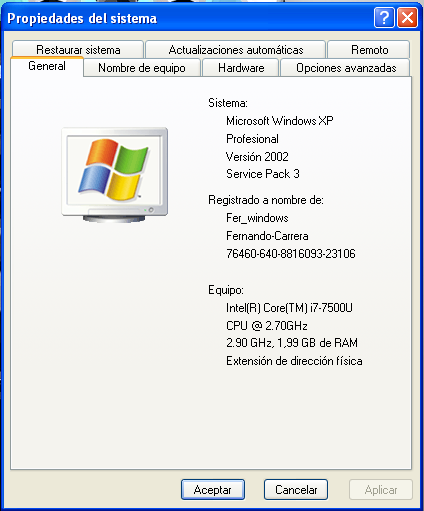
\includegraphics[width = \columnwidth]{Propiedades_windows.png}
\caption{Propiedades de la máquina virtual de windows XP - 64 bits.}
\label{Propiedades_xp}
\end{figure}

A continuación se procedió a instalar Matlab 6.5 en la máquina virtual.\\

\begin{figure}[H]
\centering
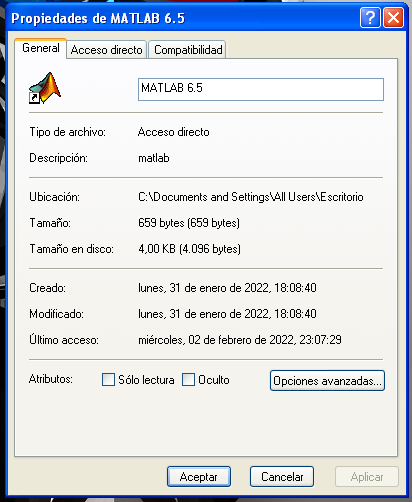
\includegraphics[width = \columnwidth]{Propiedades_matlab.png}
\caption{Propiedades Matlab 6.5.}
\end{figure}

A continuación se se configura el SIIS (Servicios de internet informatico server), el la máquina virtual y crear dos directorios virtuales nombrados, prueba y icons.\\


\begin{figure}[H]
\centering
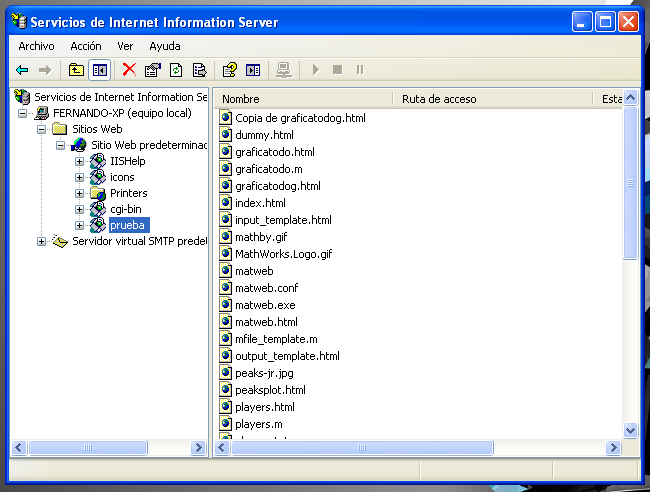
\includegraphics[width = \columnwidth]{SIIS.png}
\caption{Configuración SIIS.}
\label{SIIS}
\end{figure}

Para el directorio virtual icons, se seleccionaron las siguientes configuraciónes:\\

\begin{figure}[H]
\centering
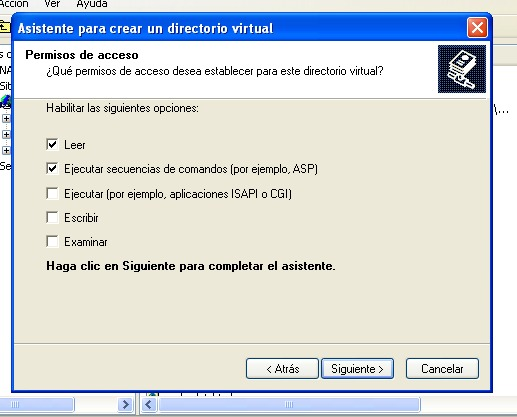
\includegraphics[width = \columnwidth]{icons.jpeg}
\caption{Configuración directorio virtual icons.}
\label{SIIS}
\end{figure}


Para el directorio virtual prueba, se seleccionaron las siguientes configuraciónes:\\

\begin{figure}[H]
\centering
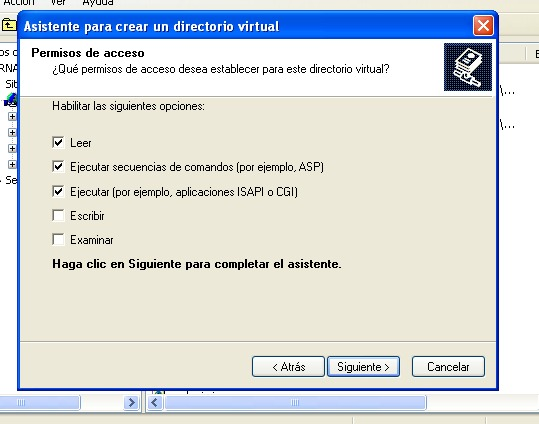
\includegraphics[width = \columnwidth]{prueba.jpeg}
\caption{Configuración directorio virtual prueba.}
\label{SIIS}
\end{figure}


Se procedió a agregar los archivos graficatodo.html, graficatodo.m y graficatodog.html, también se modificó el archivo matweb.\\

\begin{figure}[H]
\centering
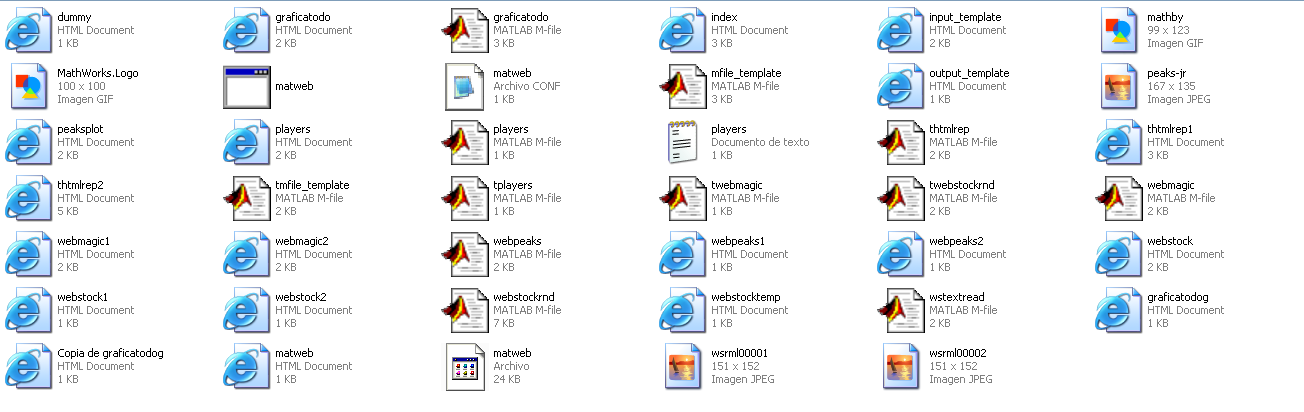
\includegraphics[width = \columnwidth]{wsdemos.png}
\caption{Carpeta wsdemos.}
\label{wsdemos}
\end{figure}

Detuvimos e iniciamos nuevamente el Mat Web Server en las opciónes de servicio en la máquina virtual.\\

\begin{figure}[H]
\centering
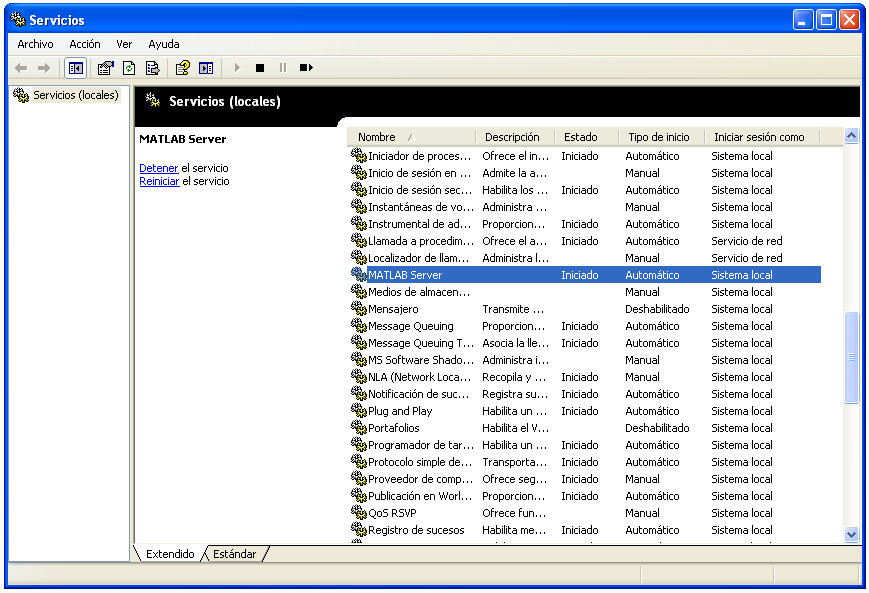
\includegraphics[width = \columnwidth]{Servicios.png}
\caption{Configuración de Servicios.}
\label{Servicios}
\end{figure}

Y por último se obtuvieron los siguientes resultados del programa graficatodo.\\

\begin{figure}[H]
\centering
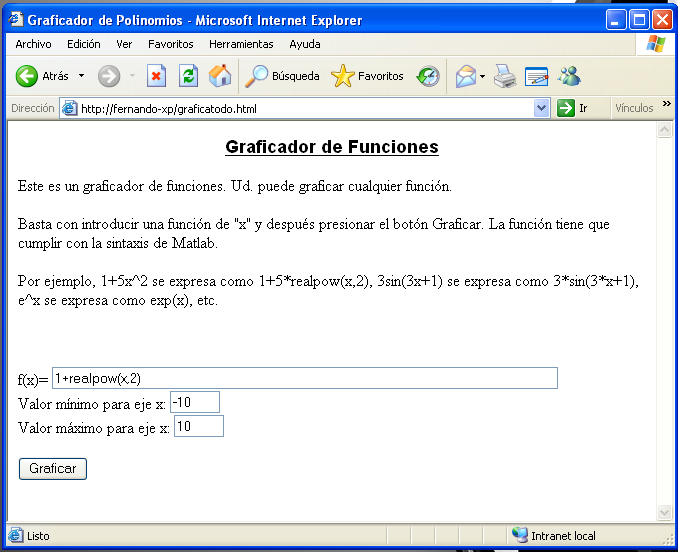
\includegraphics[width = \columnwidth]{graficador_in.png}
\caption{Pantalla en el cuál se ingresa la función a graficar.}
\label{graficador_in}
\end{figure}

\begin{figure}[H]
\centering
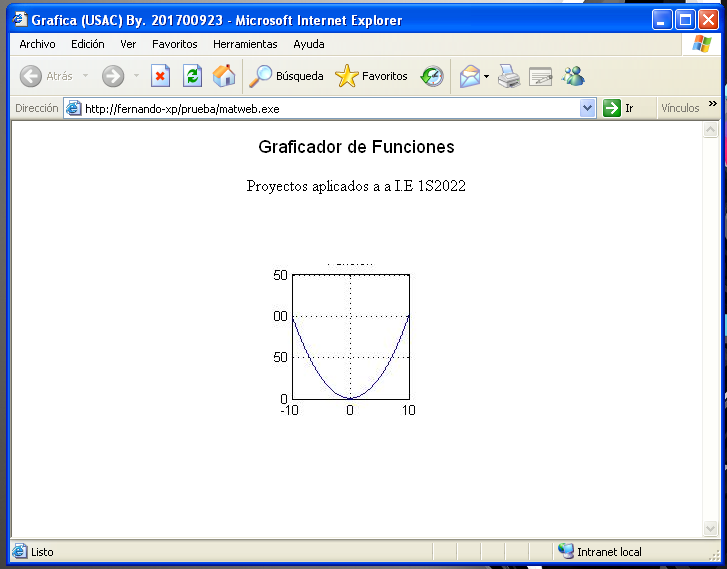
\includegraphics[width = \columnwidth]{graficador_out.png}
\caption{Pantalla con la grafica resultante.}
\label{graficador_out}
\end{figure}

\end{multicols}
\balance

\section{Contenido de los archivos .html y .m}

\subsection{graficatodo.html}

\verbatiminput{graficatodo.html}

\subsection{graficatodo.m}

\verbatiminput{graficatodo.m}

\subsection{graficatodog.html}

\verbatiminput{graficatodog.html}

\subsection{index.html}

\verbatiminput{indexa.html}

\subsection{matweb.conf}

\verbatiminput{matweba.conf}

\end{document}

